\documentclass[tikz,border=10pt]{standalone}
\usepackage{tikz}
\usetikzlibrary{positioning, arrows.meta, shapes.geometric}

\definecolor{miamired}{RGB}{200,16,46}

% Define styles for nodes
\tikzset{
	startstop/.style = {rectangle, rounded corners, draw=black, fill=miamired, text width=2.5in, text centered, minimum height=2em, font=\sffamily\bfseries, text=white},
	process/.style = {rectangle, draw=black, fill=orange!30, text width=7em, text centered, minimum height=2em, font=\sffamily},
	decision/.style = {diamond, aspect=2, draw=black, fill=green!30, text width=5em, text badly centered, inner sep=0pt, font=\sffamily},
	level0/.style = {rectangle, draw=black, very thick, text width=3cm, minimum height=1cm, text centered, font=\sffamily\bfseries},
	level1/.style = {rectangle, rounded corners, draw=black, very thick, text width=1.25in, minimum height=1cm, text centered, font=\sffamily\bfseries},
	level2/.style = {rectangle, draw=black, thick, text width=1in, minimum height=1cm, text centered, font=\sffamily},
	level3/.style = {rectangle, rounded corners, draw=miamired, thick, font=\ttfamily, text=black, align=left, inner sep=2pt, text width=1.5in, minimum height = .85cm},
	arrow/.style={-{Stealth[]}, thick},
	line/.style={draw, thick, -latex'}
}

\begin{document}
	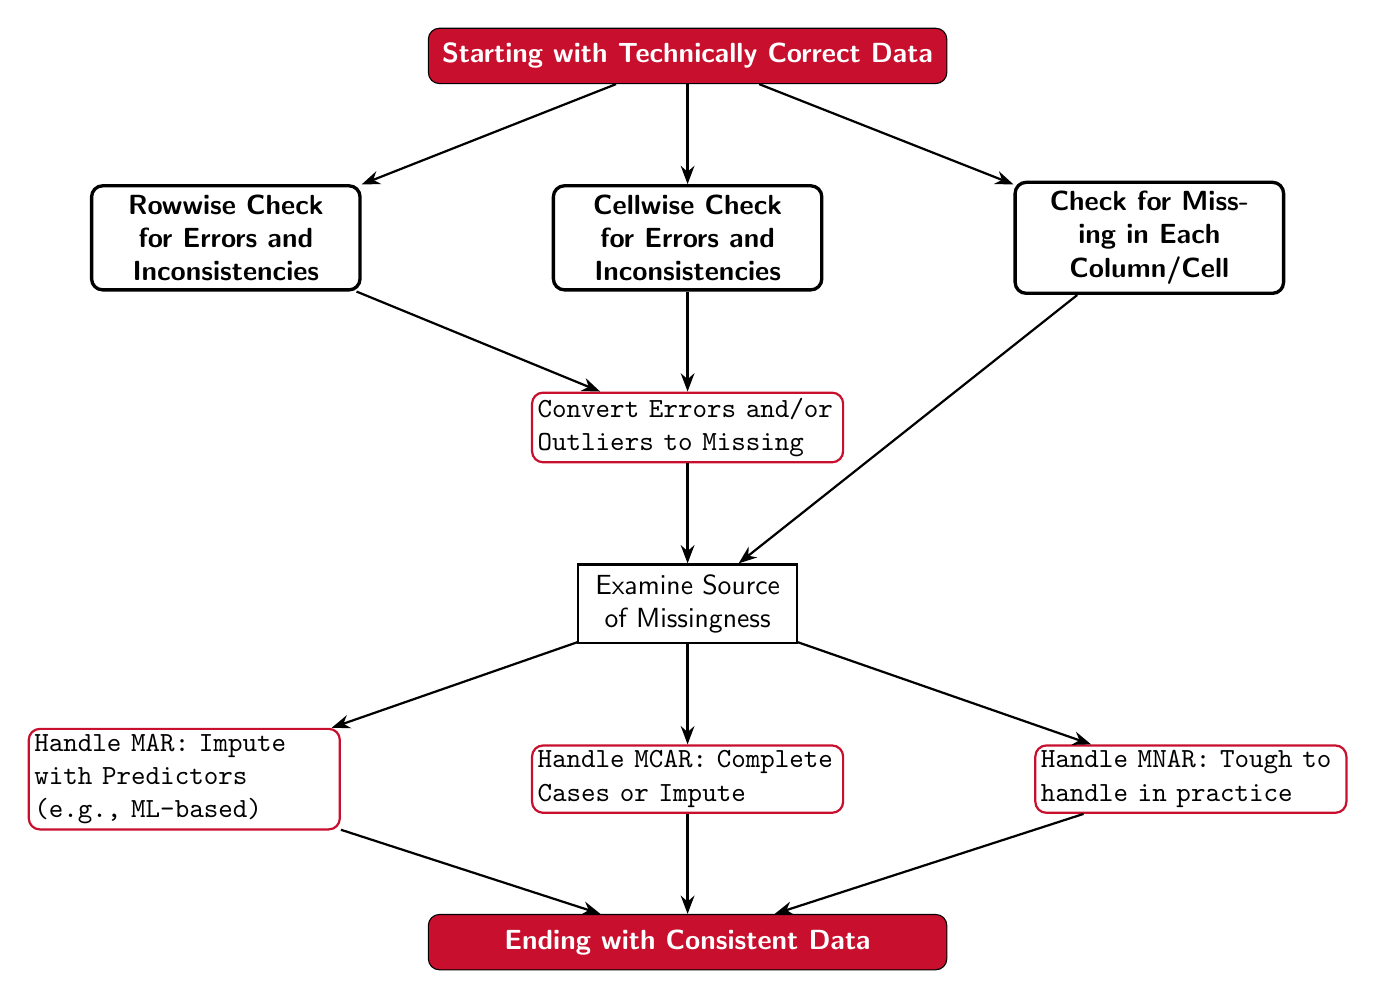
\begin{tikzpicture}[node distance=0.5in and .95in]
		
		% Start
		% Level 0: Technically Correct Data
		\node (tc_data) [startstop] {Starting with Technically Correct Data};
		
		% Level 1: Check for Errors
		\node (check_cellwise) [level1, below=of tc_data] {Cellwise Check for Errors and Inconsistencies};
		\node (check_rowwise) [level1, left=of check_cellwise] {Rowwise Check for Errors and Inconsistencies};
		\node (check_missing) [level1, right=of check_cellwise] {Check for Missing in Each Column/Cell};
		
		% Level 2: Check for Errors        
		\node (detected_outliers) [level3, below=of check_cellwise] {Convert Errors and/or Outliers to Missing};
		
		\node (source_missingness) [level2, below=of detected_outliers] {Examine Source of Missingness};
		
		% Level 3: 
		\node (handle_mcar) [level3, below=of source_missingness] {Handle MCAR: Complete Cases or Impute};
		\node (handle_mar) [level3, left=of handle_mcar] {Handle MAR: Impute with Predictors (e.g., ML-based)};
		\node (handle_mnar) [level3, right=of handle_mcar] {Handle MNAR: Tough to handle in practice};
		
		% end
		\node (end) [startstop, below=of handle_mcar] {Ending with Consistent Data};
		
		% Arrows
		\draw [arrow] (tc_data) -- (check_missing);
		\draw [arrow] (tc_data) -- (check_cellwise);
		\draw [arrow] (tc_data) -- (check_rowwise);
		\draw [arrow] (check_missing) -- (source_missingness);
		\draw [arrow] (check_cellwise) -- (detected_outliers);
		\draw [arrow] (check_rowwise) -- (detected_outliers);
		\draw [arrow] (detected_outliers) -- (source_missingness);
		\draw [arrow] (source_missingness) -- (handle_mcar);
		\draw [arrow] (source_missingness) -- (handle_mar);
		\draw [arrow] (source_missingness) -- (handle_mnar);
		\draw [arrow] (handle_mcar) -- (end);
		\draw [arrow] (handle_mar) -- (end);
		\draw [arrow] (handle_mnar) -- (end);
		
	\end{tikzpicture}
	
	
\end{document}
